% !TeX spellcheck = en_US
\documentclass[12pt, a4paper]{report}
\usepackage[scaled]{helvet}
\renewcommand\familydefault{\sfdefault}
\usepackage[T1]{fontenc}
\usepackage[margin=0.5in]{geometry}
\usepackage{float}
\usepackage{framed}
\usepackage{multicol}
\usepackage{amsmath}
\usepackage[framemethod=TikZ]{mdframed}
\usepackage{graphicx}
\usepackage{enumitem}
\usepackage{gensymb}
\setlist{nosep}
\usepackage{booktabs}
\usepackage{tikzsymbols}
\usepackage{hyperref}
\hypersetup{
	colorlinks,
	citecolor=black,
	filecolor=black,
	linkcolor=black,
	urlcolor=black
}
\usepackage{multirow}
\usepackage{pgf-umlsd}

\newcounter{note}\setcounter{note}{0}
\renewcommand{\thenote}{\arabic{note}}
\newenvironment{note}[1]{
	\stepcounter{note}
	\ifstrempty{#1}{
		\mdfsetup{
			frametitle={
				\tikz[baseline=(current bounding box.east),outer sep=0pt]
				\node[anchor=east,rectangle,fill=blue!20]
				{\strut Note~\thenote};
			}
		}
	}{
		\mdfsetup{
			frametitle={
				\tikz[baseline=(current bounding box.east),outer sep=0pt]
				\node[anchor=east,rectangle,fill=blue!20]
				{\strut Note~\thenote:~#1};
			}
		}
	}
	\mdfsetup{innertopmargin=0pt,linecolor=blue!20,linewidth=2pt,topline=true,frametitleaboveskip=\dimexpr-\ht\strutbox\relax}
	\begin{mdframed}[]\relax
}{
	\end{mdframed}
}
\newenvironment{code}{\ttfamily}{\par}

\begin{document}
	\tableofcontents
	\vspace{2em}
	\textbf{Contributors:}
	\begin{itemize}
		\item Daniel Fitz (Sanchez)
		\item Jake Dunn (nomad)
		\item \textit{Notes from UQAttic.net}
	\end{itemize}
	\newpage

\begin{multicols*}{2}

\chapter{Exam Structure}
\textbf{Exam Is Open Book!}
\subsection{What is Covered?}
\begin{itemize}
	\item All lecture content (Weeks 1, 2, 3, 5), (Required text book reading)
	\item All Seminars
	\begin{itemize}
		\item For seminars that are based on a research paper (\#20 - \#50), both content on slides and paper is relevant
		\item For all other seminars, only information presented in seminar is covered by exam
		\item Emphasis in exam will be on seminars based on research papers
	\end{itemize}
	\item Guest Lecture by Peter Robinson (W4) is not covered
\end{itemize}
\subsection{Format}
Two parts with total $\approx$ 55 marks
\begin{itemize}
	\item Part A: 8 Questions ($\approx$25 marks)
	\begin{itemize}
		\item Questions on Lectures
		\item Material covered in lectures in weeks 1,2,3 and 5
		\item Short Answer/Problem
	\end{itemize}
	\item Part B: Answer 3 questions (30 marks)
	\begin{itemize}
		\item Questions on Seminar Presentations
		\item Mix of essay-style and short answer questions
		\item Select and answer 3 out of 4 questions
		\item Cannot do own seminar question, get an extra question to choose from
	\end{itemize}
\end{itemize}
\subsubsection{Part B Example Questions}
\begin{itemize}
	\item Describe what the XREP protocol presented in the paper tries to achieve, and discuss the basic mechanisms that it is using
	\item Further discuss for what environments it can be applied and describe its limitations and vulnerabilities
	\item Describe the relevance of the parameter $K$ in the proposed protocol
	\item Describe at a high level what Aurasium is, and the key goals it is trying to achieve
	\item Describe how Aurasium interacts with the Andriod system and applications
	\item Describe if and how malicious application can detect the presence of Aurasium
\end{itemize}

\chapter{Lecture Notes}
% !TeX spellcheck = en_US
% !TeX root = notes.tex
\begin{itemize}
	\item billions of connected computing devices
	\item transmission rate: \textbf{bandwidth}
	\item \textbf{Packet Switches:} Forward packets
	\begin{itemize}
		\item \textbf{routers} and \textbf{switches}
	\end{itemize}
	\item \textbf{Internet: ``network of networks''} (Interconnected ISPs)
	\item \textbf{Protocols} control sending, receiving (e.g. TCP, IP, HTTP, Skype, 802.11)
	\item \textbf{Internet standards}
	\begin{description}
		\item[RFC:] Request for comments
		\item[IETF:] Internet Engineering Task Force
	\end{description}
\end{itemize}

\subsection{Network Structure}
\begin{itemize}
	\item \textbf{Network Edge}
	\begin{itemize}
		\item hosts: clients and servers
		\item servers often in data centers
	\end{itemize}
	\item \textbf{Access networks, physical media:} wired, wireless communication links
	\item \textbf{network core:}
	\begin{itemize}
		\item interconnected routers
		\item network of networks
	\end{itemize}
\end{itemize}

\subsection{Access Network}
\subsubsection{Digital Subscriber Line (DSL)}
\begin{itemize}
	\item use \textbf{existing} telephone line to central office DSLAM
	\begin{itemize}
		\item data over DSL phone line goes to Internet
		\item voice over DSL phone line goes to telephone net
	\end{itemize}
	\item < 2.5 Mbps upstream transmission rate (typically < 1 Mbps)
	\item < 24 Mbps downstream transmission rate (typically < 10 Mbps)
\end{itemize}
\subsubsection{Cable Network}
\begin{leftbar}
	\textbf{frequency division multiplexing:} different channels transmitted in different frequency bands
\end{leftbar}
\begin{itemize}
	\item \textbf{HFC: hybrid fiber coax}
	\begin{itemize}
		\item asymmetric: up to 30Mbps downstream transmission rate, 2 Mbps upstream transmission rate
	\end{itemize}
	\item \textbf{network} of cable, fiber attaches homes to ISP router
	\begin{itemize}
		\item homes \textbf{share access network} to cable head-end
		\item unlike DSL, which has dedicated access to central office
	\end{itemize}
\end{itemize}
\textbf{wireless LANS:}
\begin{itemize}
	\item within building (30 meters)
	\item 802.11b/g/n (WiFi): 11,54,450 Mbps transmission rate
\end{itemize}
\textbf{wide-area wireless access:}
\begin{itemize}
	\item provided by telco (cellular) operator, 10's km
	\item between 1 and 10 Mbps
	\item 3G, 4G, LTE
\end{itemize}

\subsection{Sending}
\begin{itemize}
	\item takes application message
	\item breaks into smaller chunks, known as \textbf{packets}, of length \textbf{$L$} bits
	\item transmites packet into access network at \textbf{transmission rate $R$}
	\begin{itemize}
		\item link transmission rate, aka link \textbf{capacity, aka link bandwidth}
	\end{itemize}
\end{itemize}
\begin{note}{Packet Transmission Delay}
	\[
		\text{\parbox{2cm}{packet transmission delay}}=\text{\parbox{2cm}{time needed to transmit $L$-bit packet into link}}=\frac{L\text{ (bits)}}{R\text{ (bits/sec)}}
	\]
\end{note}

\subsection{Physical Media}
\begin{itemize}
	\item \textbf{bit:} propagates between transmitter/receiver pairs
	\item \textbf{physical link:} what lies between transmitter and receiver
	\item \textbf{guided media:} signals propagate in solid media (copper, fiber, coax)
	\item \textbf{unguided media:} signals propagate freely, e.g. radio
	\item \textbf{twisted pair (TP):} two insulated copper wires
	\begin{itemize}
		\item Category 5: 100 Mbps, 1 Gbps Ethernet
		\item Category 6: 10 Gbps
	\end{itemize}
\end{itemize}
\subsubsection{Coax}
\begin{itemize}
	\item two concentric copper conductors
	\item bidirectional
	\item broadband: multiple channels on cable, HFC
\end{itemize}
\subsubsection{Fiber Optic Cable}
\begin{itemize}
	\item glass fiber carrying light pulses, each pulse a bit
	\item high-speed operation: high-speed point-to-point transmission (e.g. 10's - 100's Gbps transmission rate)
	\item low error rate
	\begin{itemize}
		\item repeaters spaced far apart
		\item immune to electromagnetic noise
	\end{itemize}
\end{itemize}
\subsubsection{Radio}
\begin{itemize}
	\item signal carried in electromagnetic spectrum
	\item no physical "wire"
	\item bidirectional
	\item propagation environment effects:
	\begin{itemize}
		\item reflection
		\item obstruction by objects
		\item interference
	\end{itemize}
\end{itemize}
\textbf{Radio Link Types:}
\begin{itemize}
	\item \textbf{terrestrial microwave:} up to 45 Mbps channels
	\item \textbf{LAN} (e.g. WiFi) 54 Mbps
	\item \textbf{wide-area} (e.g. cellular) 4G cellular: \~ 10 Mbps
	\item \textbf{satellite}
	\begin{itemize}
		\item Kbps to 45 Mbps channel (or multiple smaller channels)
		\item 270 msec end-end delay
		\item geosynchronous versus low altitude
	\end{itemize}
\end{itemize}

\subsection{Packet-switching}
\subsubsection{Store-and-forward}
\begin{leftbar}
	$L$ bits per packet\\
	Source to destination: $R$ bps
\end{leftbar}
\begin{itemize}
	\item takes $\frac{L}{R}$ seconds to transmit (push out) $L$-bit packet into link at $R$ bps
	\item \textbf{store and forward:} entire packet must arrive at router before it can be transmitted on next link
\end{itemize}
\begin{note}{End-End delay}
	\[
		\text{delay} = 2\frac{L}{R}
	\]
	(assuming zero propagation delay)
\end{note}
\subsubsection{Packet switching versus circuit switching}
Is packet switching a ``slam dunk winner?''
\begin{itemize}
	\item great for bursty data (resource sharing, simpler, no call setup)
	\item excessive congestion possible: packet delay and loss (protocols needed for reliable data transfer, congestion control)
\end{itemize}

\subsection{Packet Loss}
\begin{figure}[H]
	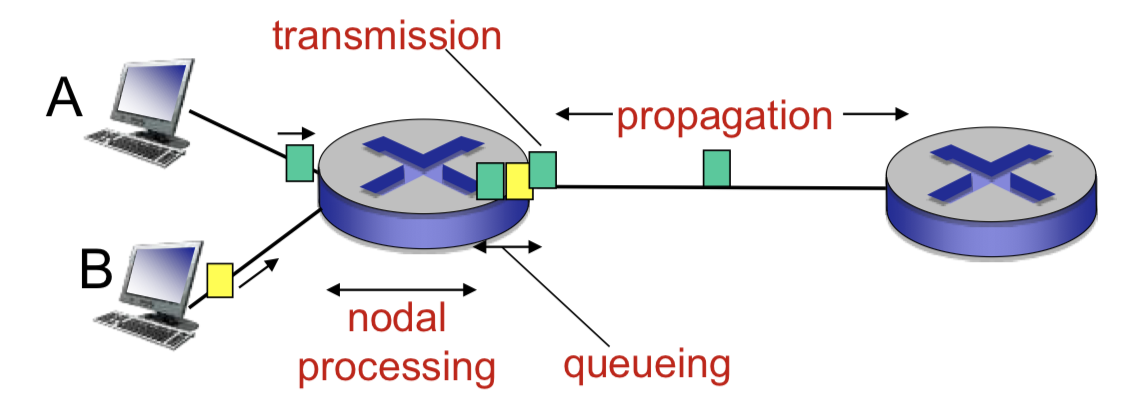
\includegraphics[width=8cm]{delay}
	\centering
	\caption{Packet Delay Algorithm Explanation}
\end{figure}
\begin{note}{Packet Delay Algorithm}
	\[ d_\text{nodal} = d_\text{proc} + d_\text{queue} + d_\text{trans} + d_\text{prop} \]
\end{note}
\subsubsection{Nodal Processing}
\[ d_\text{proc} \]
\begin{itemize}
	\item check bit errors
	\item determine output link
	\item typically < msec
\end{itemize}
\subsubsection{Queuing Delay}
\[ d_\text{queue} \]
\begin{itemize}
	\item time waiting at output link for transmission
	\item depends on congestion level of router
\end{itemize}
\subsubsection{Transmission Delay}
\[ d_\text{trans} \]
\begin{itemize}
	\item $L$: packet length (bits)
	\item $R$: link bandwidth(bps)
	\item $d_\text{trans} = \frac{L}{R}$
\end{itemize}
\subsubsection{Propagation Delay}
\[ d_\text{prop} \]
\begin{itemize}
	\item $d$: length of physical link
	\item $s$: propagation speed ($\approx2\times10^8$ m/sec)
	\item $d_\text{prop} = \frac{d}{s}$
\end{itemize}

\subsection{Throughput}
\begin{leftbar}
	Rate (bits/time unit) at which bits transferred between sender/receiver
\end{leftbar}
\begin{description}
	\item[Instantaneous:] rate at given point in time
	\item[Average:] rate over longer period of time
\end{description}
\begin{note}{Bottleneck Link}
	Link on end-end path that constrains end-end throughput
\end{note}

\subsection{Layering}
\subsubsection{Why Layering?}
Dealing with complex systems:
\begin{itemize}
	\item Explicit structure allows identification, relationship of complex system's pieces (layered \textbf{reference model} for discussion)
	\item Modularization eases maintenance, updating system
	\begin{itemize}
		\item change of implementation of layer's service transparent to rest of system
		\item e.g. change in gate procedure doesn't affect rest of system
	\end{itemize}
	\item layering considered harmful?
\end{itemize}
\subsubsection{Internet Protocol Stack}
\begin{description}
	\item[Application:] supporting network applications (FTP, SMTP, HTTP)
	\item[Transport:] process-process data transfer (TCP, UDP)
	\item[Network:] routing of datagrams from source to destination (IP, routing protocols)
	\item[Link:] data transfer between neighboring network elements (Ethernet, 802.111 (WiFi), PPP)
	\item[Physical:] bits ``on the wire''
\end{description}
\subsubsection{ISO/OSI Reference Model}
Internet stack ``missing'' these layers. These services, if needed, must be implemented in application.
\begin{description}
	\item[Application:]
	\item[Presentation:] allow applications to interpret meaning of data, e.g. encryption, compression, machine-specific conventions
	\item[Session:] synchronization, check-pointing, recovery of data exchange
	\item[Transport:]
	\item[Network:]
	\item[Link:]
	\item[Physical:]
\end{description}

\subsection{Security}
\begin{itemize}
	\item Malware can get in host from:
	\begin{description}
		\item[Virus:] self-replicating infection by receiving/executing object (e.g. e-mail attachment)
		\item[Worm:] self-replicating infection by passively receiving object that gets itself executed
	\end{description}
	\item \textbf{Spyware malware} can record keystrokes, web sites visited, upload info to collection site
	\item Infected host can be enrolled in \textbf{botnet}, used for spam. DDoS attacks
\end{itemize}
\subsubsection{DoS: Denial of Service}
\textbf{Denial of Service (DoS):} attackers make resources (server, bandwidth) unavailable to legitimate traffic by overwhelming resource with bogus traffic
\begin{enumerate}
	\item select target
	\item break into hosts around the network (botnet)
	\item send packets to target from compromised hosts
\end{enumerate}
\subsubsection{Sniffing}
\begin{itemize}
	\item broadcast media (shared Ethernet, wireless)
	\item promiscuous network interface reads/records all packets (e.g. including passwords) passing by
\end{itemize}
\subsubsection{IP Spoofing}
Send packet with false source address
% !TeX spellcheck = en_US
% !TeX root = notes.tex
\subsection{Application Architectures}
\subsubsection{Client-Server}
\begin{description}
	\item[Server:] Always-on host, Permanent IP address
	\item[Clients:] Do not communicate directly with each other, May have dynamic IP addresses
\end{description}

\subsubsection{Peer-to-Peer (P2P)}
\begin{itemize}
	\item No always-on server
	\item Peers request service from other peers, provide service in return to other peers
	\item \textbf{Self Scalability} -- new peers bring new service capacity, as well as new service demands
	\item Pers are intermittently connected and change IP addresses
\end{itemize}

\begin{note}{App-layer protocol defines}
	\begin{itemize}
		\item \textbf{type of messages exchanged} -- e.g. request, response
		\item \textbf{message syntax} -- what fields in messages and how fields are delineated
		\item \textbf{message semantics} -- meaning of information in fields
		\item \textbf{rules} for when and how processes send and respond to messages
		\item \textbf{open protocols} -- defined in RFCs, allows for interoperability (e.g. HTTP, SMTP)
		\item \textbf{proprietary protocols} -- e.g. Skype
	\end{itemize}
\end{note}

\subsection{Transport Service is needed}
\begin{description}
	\item[Data Integrity:] Some programs need 100\% reliable data transfer (e.g. file transfer, web transactions), others can tolerate loss (e.g. audio)
	\item[Timing:] Some programs require low delay to be ``effective'' (e.g. online games)
	\item[Throughput:] Some programs require minimum amount of throughput to be ``effective'' (e.g. multimedia), some use whatever they have available (``elastic apps'')
	\item[Security:] Encryption, Data Integrity
\end{description}

\subsection{Transport Protocol Services}
\subsubsection{TCP}\label{sec:tcp}
\begin{description}
	\item[Reliable Transport] between sending and receiving process
	\item[Flow Control:] sender won't overwhelm receiver
	\item[Congestion Control:] throttle sender when network overloaded
	\item[Connection-Oriented:] setup required between client and server processes
	\item[Does Not Provide:] timing, minimum throughput guarantee, security
\end{description}

\subsubsection{UDP}\label{sec:udp}
\begin{description}
	\item[Unreliable Data Transfer] between sending and receiving process
	\item[Does Not Provide:] reliability, flow control, congestion control, timing, throughput guarantee, security, or connection setup
\end{description}

\subsubsection{Securing TCP}
\textbf{TCP and UDP}
\begin{itemize}
	\item no encryption
	\item cleartext passwords sent into socket traverse Internet in cleartext
\end{itemize}
\textbf{SSL}
\begin{itemize}
	\item provides encrypted TCP connection
	\item data integrity
	\item end-point authentication
\end{itemize}
\textbf{SSL is at app layer}
\begin{itemize}
	\item app use SSL libraries, that ``talk'' to TCP
\end{itemize}
\textbf{SSL socket API}
\begin{itemize}
	\item cleartext passwords sent into socket traverse Internet encrypted
\end{itemize}

\subsection{HTTP: Hypertext Transfer Protocol}\label{sec:http}
\begin{itemize}
	\item Web's application layer protocol
	\item client/server model. Client request website and server serves HTTP object in response
	\item Uses TCP
	\item HTTP is stateless. Server maintains no information about past client requests
	\item \textbf{non-persistent HTTP:} one object sent over one TCP connection, downloading multiple object required multiple connections
	\item \textbf{persistent HTTP:} multiple object sent over single TCP connection
\end{itemize}
Non-persistent HTTP issues:
\begin{itemize}
	\item requires 2 RTTs per object
	\item OS overhead for each TCP connection
	\item browsers often open parallel TCP connections to fetch referenced objects
\end{itemize}
Persistent HTTP:
\begin{itemize}
	\item server leaves connection open after sending response
	\item subsequent HTTP messages between same client/server sent over open connection
	\item client sends requests as soon as it encounters a referenced object
	\item as little as one RTT for all the referenced objects
\end{itemize}
\subsubsection{Method Types}
\textbf{HTTP/1.0:} GET, POST, HEAD (asks server to leave requested object out of response)\\
\textbf{HTTP/1.1:} GET, POST, HEAD, PUT (uploads file in entity body to path specified in URL field), DELETE (deletes file specified in the URL field)
\subsubsection{Response Codes}
\begin{description}
	\item[200 OK:] request succeeded, requested object later in this msg
	\item[301 Moved Permanently:] requested object moved, new location specified later in this msg
	\item[400 Bad Request:] request msg not understood by server
	\item[404 Not Found:] requested document not found on this server
	\item[505 HTTP Version Not Supported]
\end{description}

\subsection{Cookies}
Uses: authorization, shopping carts, recommendations, user session state (Web, email)

\subsection{Web Caches (proxy server)}
\begin{leftbar}
	\textbf{Goal:} satify client request without involving origin server
\end{leftbar}
\begin{itemize}
	\item Browsers requests object from cache, if in cache the object is sent back otherwise cache requests object from origin
	\item Cache acts as both client and server
	\item Reduce response time for client request
	\item Reduce traffic
\end{itemize}

\subsubsection{Conditional GET}
\begin{leftbar}
	\textbf{Goal:} don't send object if cache has up-to-date cached version (lower link usage)
\end{leftbar}
\begin{itemize}
	\item \textbf{Cache:} specify date of cached copy in HTTP request \texttt{If-modified-since: <date>}
	\item \textbf{Server:} response contains no object if cached copy is up-to-date: \texttt{HTTP/1.0 Not Modified}
\end{itemize}

\subsection{Electronic Mail: SMTP}\label{sec:smtp}
\textit{RFC 2821}
\begin{itemize}
	\item uses TCP to reliably transfer email message from client to server, port 25
	\item direct transfer: sending server to receiving server
	\item three phases of transfer: handshaking, transfer of messages, closure
	\item command/response interaction
	\item messages must be in 7-bit ASCII
	\item uses persistent connections
	\item requires message to be in 7-bit ASCII
	\item uses \texttt{CRLF.CRLF} to determine end of message
\end{itemize}
Difference to HTTP being, HTTP is server sending data, SMTP is client connection sending data\\
\begin{description}
	\item[SMTP:] protocol for exchanging email messages
	\item[RFC 822:] standard for text message format (To, From, Subject, Body)
\end{description}
\subsubsection{Mail Access Protocols}
\begin{leftbar}
	\textbf{SMTP:} delivery/storage to receiver's server
\end{leftbar}
\begin{description}
	\item[POP:] Post Office Protocol \textit{(RFC 1939)}: authorization, download
	\begin{itemize}
		\item POP3 is stateless across sessions
		\item Two main modes; download and delete, download and keep (allows multiple clients to read the same email)
	\end{itemize}
	\item[IMAP:] Internet Mail Access Protocol \textit{(RFC 1730)}: more features, including manipulation of stored message on server
	\begin{itemize}
		\item All messages stored on server
		\item Supports folders
		\item Keeps user state across sessions: names of folders and mappings between message IDs and folder name
	\end{itemize}
	\item[HTTP:] gmail, Hotmail, Yahoo, etc
\end{description}

\subsection{DNS: Domain Name System}\label{sec:dns}
\begin{itemize}
	\item Lookup between names (e.g. google.com) and IP addresses
	\item \textbf{Distributed Database} implemented in hierarchy of many \textbf{name servers}
	\item \textbf{Application-layer protocol:} hosts, name servers communicate to \textbf{resolve} names (address/name translation)
\end{itemize}
Why not centralize DNS? Single point of failure, traffic volume, doesn't scale
\subsubsection{DNS Services}
\begin{itemize}
	\item hostname to IP address translation
	\item host aliasing (canonical, alias names)
	\item mail server aliasing
	\item load distribution (many IP addresses correspond to one name)
\end{itemize}
\subsubsection{TLD, authoritative servers}
\textbf{top-level domain (TLD) servers:}
\begin{itemize}
	\item responsible for com, org, net, edu, aero, jos, io
	\item and top-level country domains au, uk, ca
	\item Network Solutions maintains servers for .com TLD
	\item Educause for .edu TLD
\end{itemize}
\textbf{Authoritative DNS servers:}
\begin{itemize}
	\item organization's own DNS server(s), providing authorative hostname to IP mappings for organization's named hosts
	\item can be maintained by organization or service provider
\end{itemize}
\subsubsection{Local DNS name server}
\begin{itemize}
	\item does not strictly belong to hierarchy
	\item each ISP (residential ISP, company, university) has one (also called ``default name server'')
	\item when host makes DNS query, query is sent to its local DNS server
	\begin{itemize}
		\item has local cache of recent name-to-address translation pairs (but may be out of date!)
		\item acts as proxy, forwards query into hierarchy
	\end{itemize}
\end{itemize}
\subsubsection{DNS Name Resolution}
\begin{description}
	\item[Iterated query:] contacted server replies with name of server to contact. So root dns sends the ip of the next dns server to contact
	\item[Recursive query:] puts burden of name resolution on contacted name server. So root dns server contacts the next levels down which contacts next level down.
\end{description}
\subsubsection{Caching}
Once (any) name server learns mapping, it \textbf{caches} mapping. Cache entries timeout (disappear) after some time (TTL). If name host changes IP address, the name servers might not update until TTLs expire.
\begin{leftbar}
	update/notify mechanisms proposed IETF standard RFC 2136
\end{leftbar}
\subsubsection{DNS Records}
\begin{note}{RR Format}
	\texttt{(name, value, type, ttl)}
\end{note}
\begin{description}
	\item[type=A] \texttt{name} is hostname, \texttt{value} is IP address
	\item[type=NS] \texttt{name} is domain (e.g. google.com), \texttt{value} is hostname of authoritative name server for this domain
	\item[type=CNAME] \texttt{name} is alias name for some ``canonical'' (the real) name (\texttt{www.ibm.com} is really \texttt{servereast.backup2.ibm.com}), \texttt{value} is canonical name
	\item[type=MX] \texttt{value} is name of mailserver associated with \texttt{name}
\end{description}
\subsubsection{Protocol}
Query and reply messages both follow same format
\begin{table}[H]
\centering
\caption{Protocol Layout}
\begin{tabular}{cc}
	\toprule
	2 bytes & 2 bytes \\
	\midrule
	identification & flags\\
	\# questions & \# answer RRs\\
	\# authority RRs & \# additional RRs\\
	\multicolumn{2}{c}{questions (variable \# of questions)}\\
	\multicolumn{2}{c}{answers (variable \# of RRs)}\\
	\multicolumn{2}{c}{authority (variable \# of RRs)}\\
	\multicolumn{2}{c}{additional info (variable \# of RRs)}\\
	\bottomrule
\end{tabular}
\end{table}
\subsubsection{Attacking DNS}
\textbf{DDoS attacks}
\begin{itemize}
	\item bombard root servers with traffic. Not successful to date, traffic filtering, local DNS servers cache protecting root DNS
	\item bombard TLD server. Potentially more dangerous
\end{itemize}
\textbf{Redirect Attacks}
\begin{itemize}
	\item man-in-middle (Intercept queries)
	\item DNS Poisoning (Send bogus relies to DNS server, which caches)
\end{itemize}
\textbf{Exploit DNS for DDoS}
\begin{itemize}
	\item send queries with spoofed source address: target IP
	\item requires amplification
\end{itemize}
% !TeX spellcheck = en_US
% !TeX root = notes.tex
\section{Lecture 3: Bitcoin, Cryptocurrencies Blockchain Technology}
\subsection{Sybil Attack}
\begin{itemize}
	\item The Sybil attack in computer security is an attack wherein a reputation system is subverted by forging identities in peer-to-peer networks.
	\item Creates a large number of false identities in order to flood the network and take it over.
	\item Named after the subject of the book \textbf{Sybil}, a case study of a woman diagnosed with multiple personality disorder
	\item Such false identities are called \textbf{``Sybils''}, in the context of P2P systems
	\item One approach to preventing these “Sybil attacks” is to have a trusted agency certify identities.
	\item Or \textbf{``Sockpuppets''} in the context of the Internet, e.g. to manipulate public opinion
	\begin{leftbar}
		``... referred to a false identity assumed by a member of an Internet community who spoke to, or about, themselves while pretending to be another person. `The term now includes other misleading uses of online identities, such as those created to praise, defend or support a person or organization, to manipulate public opinion, or to circumvent a suspension or ban from a website''\\
		- Wikipedia
	\end{leftbar}
\end{itemize}

\subsection{Decentralized Consensus in Bitcoin}
\begin{itemize}
	\item Bitcoin achieves consensus by replacing \textbf{one node (or one IP address) one vote}, with \textbf{one CPU one vote}
	\item Bitcoin mining uses mostly ASICs and GPUs, not CPUs
	\item Consensus is achieved by a (probabilistic) majority vote, based on computing power
	\begin{itemize}
		\item Attacker needs > 50\% of combined computing power in order to cheat with high probability
		\item This is harder to achieve than controlling more than half of the nodes
		\item It's relatively easy to spin up a few thousand VMs as nodes, compared to controlling >50\% of Bitcoin's mining compute power
	\end{itemize}
	\item Bitcoin combines a \textbf{proof-of-work mechanism} (based on Hashcash), combined with a clever incentive mechanism $\rightarrow$ Nodes get paid to do the right thing, i.e. checking and confirming valid transactions via ``mining''
\end{itemize}

\section{Lecture 3: Bitcoin}
\begin{itemize}
	\item Complete transaction history is stored in public ledger (blockchain), stored by nodes in P2P network
	\item New transactions are created off-line, and then broadcast is P2P network
	\item Nodes validate and relay transactions (if valid)
	\item Nodes add new transactions (not part of blockchain yet) to a \textbf{transaction pool}
	\item Nodes combine transactions in pool to a block, and try to solve the corresponding proof-of-work puzzle, to ``confirm'' the block
	\item Node that finds solution first broadcasts block with solution in the network (Winning node selection is probabilistic, with probability propertional to computing power)
	\item Nodes check solution, and if OK, add new block to their local copy of blockchain
	\item All nodes who were working on solving the old puzzle, immediately start working on a new block
	\begin{itemize}
		\item Everybody always works on the longest chain
		\item Convergence to longest chain provides consensus
		\item Forks happen but are resolved by (computational) majority vote
	\end{itemize}
\end{itemize}
\begin{note}{Bitcoin Components}
	\begin{itemize}
		\item Bitcoin Network
		\item Bitcoin Identities/Addresses
		\item Bitcoin Transactions
		\item Bitcoin Scripting Language
		\item Blocks
		\item Proof-of-work, Hash puzzles, Mining
		\item Consensus
	\end{itemize}
\end{note}

\subsection{Bitcoin Network}
Transactions are broadcast in the Bitcoin network, consisting of ``full'' Bitcoin nodes ($\approx$10,000)
\begin{itemize}
	\item Best-effort (asynchronous, unreliable), it's enough if only some nodes get the message
	\item It's easy to join the Bitcoin Network, just download and run the client (Bitcoin is a \textbf{permissionless, public} blockchain, anyone can join)
\end{itemize}
Network is unstructured P2P network (random topology)
\begin{itemize}
	\item Similar to Gnutella (a P2P system from a long time ago)
	\item Overlay network, TCP, port 8333
	\item Messages are flooded
	\item All nodes are equal, no hierarchy
	\item Nodes can join at any time
	\item Node is `forgotten' if it does not respond for more than 3 hours
	\item Network is very simple and robust, e.g. to churn, but not very efficient
\end{itemize}
\begin{note}{Bitcoin Network Nodes}
	\begin{itemize}
		\item Check validity of transactions
		\item Relay transactions in the network via flooding
		\item Mining (proof-of-work puzzles)
		\item Validate and forward confirmed blocks (Add them to local copy of blockchain)
	\end{itemize}
\end{note}
\subsection{Bitcoin Identity and Addresses}
Users are represented by their Public Key addresses (hash), called \textbf{Bitcoin Addresses}, which serve as a pseudonyms
\begin{itemize}
	\item An address is a \textbf{160 bit} value, and is computed as follows
	\item RIPEMD160 hash of SHA-256 hash of ECDSA Public Key
	\item This is a ``Pay-to-pubkey-hash (P2PKH)'' address, encoding starts with ``1''
\end{itemize}
When spending a coin, spender needs to proof ownership of coin by providing a valid digital signature on the spend transaction (i.e. proving ownership of corresponding private key)\\
How can digital signatures be verified?
\begin{itemize}
	\item We need public key, not just hash of public key
	\item Spender of coin needs to provide both valid signature AND public key
	\item How do we know the provided public key is authentic $\rightarrow$ Hash it, and compare with Bitcoin address, which is the hash of public key
\end{itemize}
Bitcoin also supports \textbf{Pay to script hash (P2SH)} addresses
\begin{itemize}
	\item Allow transactions to be sent to a \textbf{script hash} instead of a public key hash (Address encoding starts with a `3' instead of `1')
	\item To spend bitcoins sent via P2SH, the recipient must provide a script matching the script hash and data which makes the script evaluate to true
	\item Allows more complex transactions (\textbf{smart contracts}), e.g. transaction outputs that require multiple signatures (multisig), or transaction puzzle, ...
\end{itemize}
\begin{note}{Bitcoin Address Encoding}
	Bitcoin uses Base58 encoding (binary-to-text encoding). Similar to Base64 encoding, but without some characters. Rationale, as explained in original bitcoin client source code:
	\begin{code}
		// Why base-58 instead of standard base-64 encoding?\\
		// - Don't want 0OIL characters that look like the same in some fonts and\\
		//   could be used to create visually identical looking account numbers.\\
		// - A string with non-alphanumeric characters is not as easily accepted as an account nbr.\\
		// - E-mail usually won't line-break if there's no punctuation to break at.\\
		// - Doubleclicking selects the whole number as one word if it's all\\alphanumeric.
	\end{code}
	Bitcoin also adds 4 byte checksum to addresses
\end{note}
\subsubsection{Bitcoin Address -- Balance}
\begin{itemize}
	\item The ``balance'' of an address is the total of unspent transaction outputs (UTXO) sent to the address.
	\item ``There are no accounts or balances in bitcoin; there are only unspent transaction outputs (UTXO) scattered in the blockchain''
	\item A user typically has many different addresses, all managed by the ``wallet'' software
	\item The wallet ``balance'' is the sum of all unspent transaction outputs of all addresses owned by the user
\end{itemize}
\subsection{Bitcoin Transactions}
\begin{itemize}
	\item Transaction are created off-line (No need to be connected to Bitcoin network for this)
	\item Transactions are broadcast in Bitcoin P2P network
	\item Nodes check validity, and relay transaction (flooding)
	\item Nodes add to new transactions to a block and try to solve hash puzzle
	\item A block with a solved puzzle is ``confirmed'', and broadcast in the network, and added to the blockchain of each node
	\item Contains:
	\begin{itemize}
		\item Inputs (any number $\geq0$)
		\item Outputs (any number > 0)
		\item Digital signatures of input coin owners (Typically for \textbf{P2PKH} transactions)
		\item Input needs to be completely consumed (With exception of Transaction Fee)
	\end{itemize}
\end{itemize}
\subsubsection{Basic Transaction Types}
\begin{itemize}
	\item Common Transaction
	\begin{itemize}
		\item 1 input
		\item 1 ``normal'' output
		\item 1 change output (back to owner)
		\subitem Create new ``Change Address'' to maintain ``anonymity''
	\end{itemize}
	\item Aggregating Transaction
	\begin{itemize}
		\item Multiple inputs
		\item 1 output
	\end{itemize}
	\item Distributing Transaction
	\begin{itemize}
		\item 1 input
		\item Multiple outputs
	\end{itemize}
	\item ``Coinbase Transaction''
	\begin{itemize}
		\item 0 input, 1 outputs
		\item Freshly created (``minted'') coins
		\item Miner gets this as a reward for solving Hash puzzle (and thereby confirming block)
		\item First transaction in every block
	\end{itemize}
\end{itemize}

\subsection{Bitcoin Scripts}
\begin{itemize}
	\item Two types of Bitcoin scripts to validate transactions
	\begin{itemize}
		\item a locking script (Typically \textbf{ScriptPubKey})
		\item and an unlocking script (Typically \textbf{ScriptSig})
	\end{itemize}
	\item A locking script is a condition placed on an output
	\item It specifies the conditions that must be met to spend or consume the output in the future
	\begin{itemize}
		\item Typically a \textbf{valid digital signature} of the claimed owner
		\item Can be other things, to implement basic `smart contracts'
	\end{itemize}
\end{itemize}
\subsubsection{Bitcoin Scripting Language ``Script''}
\begin{itemize}
	\item Allows to program conditions required for the spending of Bitcoins (``Programmable Money'')
	\item \textbf{Script} is a simple, stack based language
	\item Not Turing complete (e.g. no loops)
	\item Scripts are guaranteed to terminate after a fixed number of steps, e.g. no infinite loops
	\item Why is this a good thing?
	\begin{itemize}
		\item Avoids potential denial of service attacks on nodes, ``logic bombs''
		\item Remember: Every node runs all scripts to validate all transactions (BTW, this severely limits scalability of Bitcoin)
	\end{itemize}
	\item In contrast, Ethereum has a Turing complete scripting language
	\subitem Solves DoS attack problem by putting a price on script computation (`Gas')
\end{itemize}

\subsection{Blocks}
\begin{itemize}
	\item Transactions are grouped into blocks
	\subitem This is an optimization. Confirming individual transactions and adding them to the blockchain would be possible, but very inefficient
	\item Transactions are stored in a Merkle Tree, with the Merkle Root (Tx\_Root) stored in the block header
	\item Once confirmed (via solving hash puzzle), a block is added to the blockchain
	\item The `Nonce' is the solution of the hash puzzle
\end{itemize}
\begin{figure}[H]
	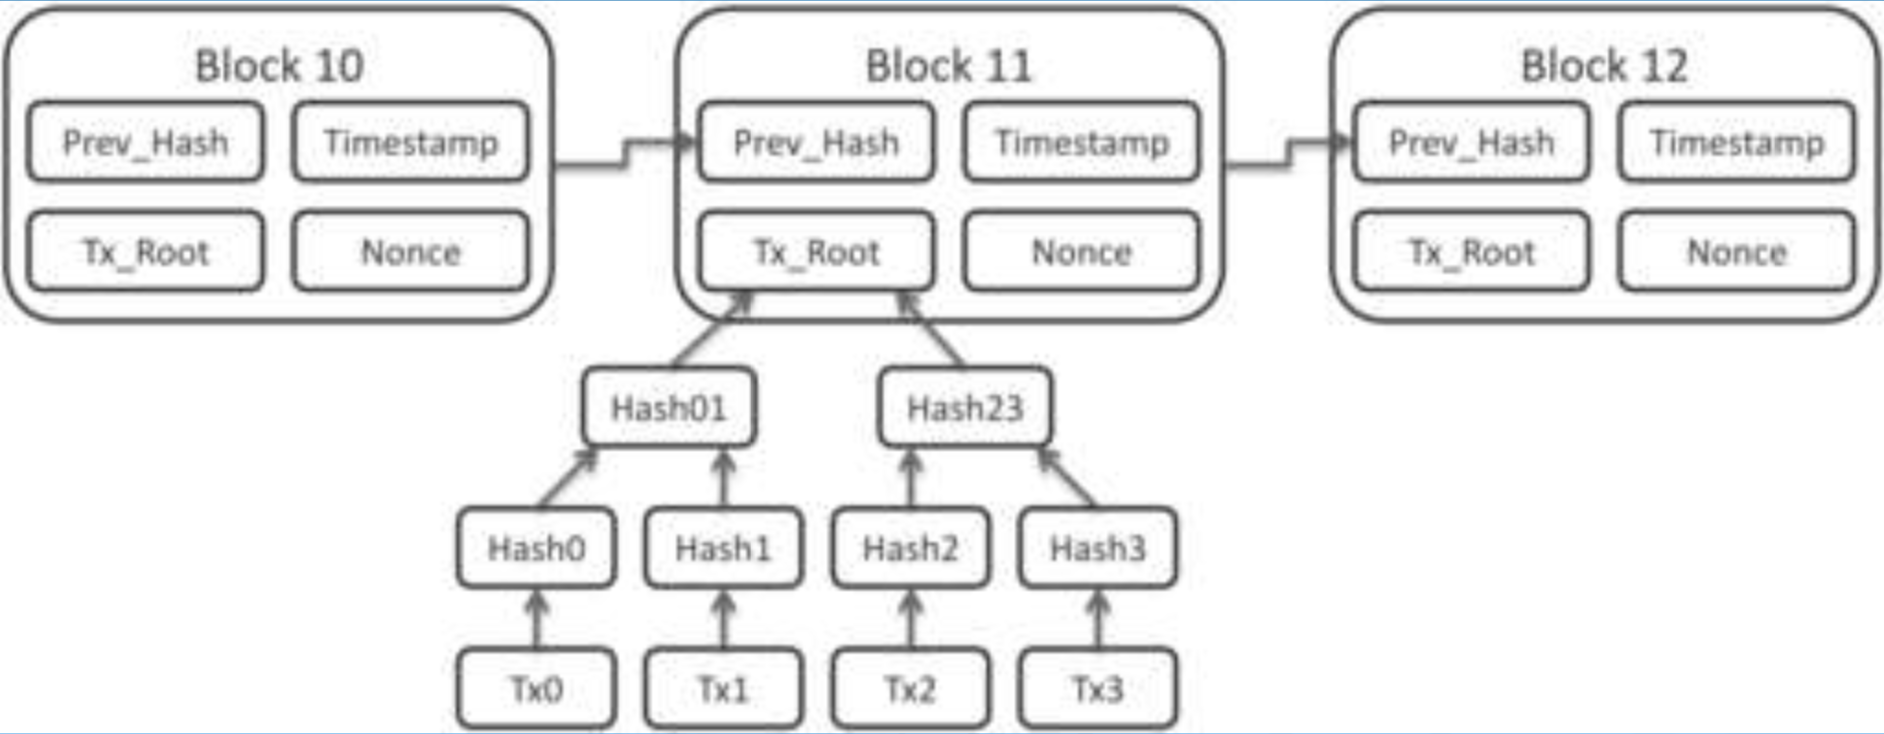
\includegraphics[width=\linewidth]{blockStructure}
	\centering
	\caption{Block Structure}
\end{figure}
\subsubsection{How are blocks added to the Blockchain?}
\begin{itemize}
	\item Multiple nodes (miners) are working towards solving the hash puzzle for a new block
	\subitem miners are probably working on different version of blocks, depending on content on their transaction pool
	\item First node who solves puzzle, broadcasts new block with solution (nonce) in the Bitcoin P2P network
	\begin{itemize}
		\item Choice of winning node is random (probabilistic)
		\item Probability of success is proportional to computing power of miner
	\end{itemize}
	\item ``Block Height'' is sequence number of blocks
	\item Other nodes check if solution is correct, and if so, add block to their local copy of the blockchain, and forward new block to other nodes
\end{itemize}

\subsection{Bitcoin Mining}
\begin{itemize}
	\item At the current level of difficulty, solving Bitcoin hash puzzles is hard and expensive
	\item Mostly ASICs based, some GPUs
	\item Total hash rate of entire Bitcoin network $\approx25\times10^{18}$H/s
	\item Hash rate of an Intel i7 CPU $\approx10$MH/s
	\subitem Need > 10,000,000 laptops to be able to mine one block per year on average
	\item Finite amount of BTC $\approx$21 Million
	\item Bitcoin is deflationary (value increases, people are potentially hoarding Bitcoin)
\end{itemize}
\subsubsection{Mining Incentive/Reward}
\begin{itemize}
	\item Transaction Fees
	\begin{itemize}
		\item Difference between total input and total output value of transaction
		\item Optional, but miners prioritize inclusion of transactions into blocks based on fees (Like giving a tip)
	\end{itemize}
	\item Block Reward
	\begin{itemize}
		\item For each solved puzzle (confirmation of block), miner currently gets freshly minted 12.5 BTC
		\item ``Coinbase transaction'' ($1^{st}$ transaction in each block)
		\item This is the only way in which coins are generated in Bitcoin
		\item Reward halved every 4 years (initially 50 BTC)
		\item Essentially no more Block Reward in 2040
	\end{itemize}
\end{itemize}

\subsection{Consensus}
\begin{itemize}
	\item Blockchain forks can happen, e.g. due to race conditions and variable latency in Bitcoin network (\textit{two nodes might find a solution to the puzzle at almost the same time}), or due to double spend attempt
	\item Nodes converge on one chain, they all aim to work on the longest (main) chain, and eventually one chain wins
	\item Incentive to work on the longest chain (Block Reward and TX fees can only be spent if block remains in the longest chain (need a certain number of \textbf{confirmations}, i.e. blocks added))
	\item Block on discontinued branches are called ``orphaned blocks''
	\item Heuristic
	\subitem Transactions are considered ``confirmed'' if they are in a block that has at least 6 blocks added to the chain (i.e. 6 confirmation) \textit{(There is nothing special about the number 6)}
	\item This means if someone wanted to reverse a transaction, they would have to go back 6 blocks, and re-do all the hash puzzles, before another nodes adds a new block at the end of chain (Practically impossible, unless attacker hash more than 50\% of computing power of entire network)
	\item Other types of attacks:
	\begin{itemize}
		\item Publish an invalid transaction, e.g. trying to spend coins that he does not own (no valid signature). Honest nodes would reject the transaction
		\item Double spend attack. Cause a fork in the chain, majority vote will guarantee that only one chain will exist
		\item Launch DoS attack against
	\end{itemize}
	\item With more than 50\% computing power, more beneficial to play by the rules and gain Block Rewards
\end{itemize}
% !TeX spellcheck = en_US
% !TeX root = notes.tex
\subsection{Transport vs. Network Layer}
\begin{description}
	\item[Network Layer:] logical communication between hosts
	\item[Transport Layer:] logical communication between processes; relies on, enhances, network layer services
\end{description}

\subsection{Multiplexing/demultiplexing}
\subsubsection{How demultiplexing works}
\begin{itemize}
	\item host receives IP datagrams
	\begin{itemize}
		\item each datagram as source IP address, destination IP address
		\item each datagram carries one transport-layer segment
		\item each segment has source, destination port number
	\end{itemize}
	\item host uses \textbf{IP addresses and port numbers} to direct segment to appropriate socket
\end{itemize}\newpage
\textbf{Connectionless Demultiplexing}
\begin{leftbar}
	A UDP socket needs to have a local port number assigned to it (both client and server)
\end{leftbar}
\textbf{Connection-oriented demux}
\begin{leftbar}
	TCP socket identified by 4-tuple: \textbf{(source IP address, source port number, dest IP address, dest port number)}
\end{leftbar}

\subsection{UDP}
\begin{table}[H]
	\centering
	\caption{UDP Segment Header}
	\begin{tabular}{cc}
		\toprule
		\multicolumn{2}{c}{32 bits}\\
		\midrule
		source port \# & dest port \#\\
		length & checksum\\
		\multicolumn{2}{c}{application data (payload)}\\
		\bottomrule
	\end{tabular}
\end{table}
\subsubsection{UDP Checksum}
\textbf{Sender:}
\begin{itemize}
	\item treat segment contents, including header fields, as sequence of 16-bit integers
	\item checksum: addition (one's complement sum) of segment contents
	\item sender puts checksum value into UDP checksum field
\end{itemize}
\textbf{Receiver:}
\begin{itemize}
	\item compute checksum of received segment
	\item check if computed checksum equals checksum field value
\end{itemize}

\subsection{Pipelined Protocols}
\begin{leftbar}
	\textbf{Pipelining:} sender allows multiple, "in-flight", yet-to-be-acknowledged packets. Range of sequence numbers must be increased, buffering at sender and/or receiver.
\end{leftbar}
\subsubsection{Go-Back-N}
\begin{itemize}
	\item sender can have up to$N$ unacked packets in pipeline
	\item receiver only sends \textbf{cumulative ack}. Doesn't ack packet if there's a gap
	\item sender has timer for oldest unacked packet. When timer expires, retransmit all unacked packets
\end{itemize}
\subsubsection{Selective Repeat}
\begin{itemize}
	\item sender can have up to $N$ unacked packets in pipeline
	\item receiver sends \textbf{individual ack} for each packet
	\item sender maintains timer for each unacked packet. When timer expires, retransmit only that unacked packet
\end{itemize}

\chapter{Paper Summaries}

% !TeX spellcheck = en_US
% !TeX root = notes.tex
\section{\#20 On Scaling Decentralized Blockchains}
\begin{itemize}
	\item Tackles the question of whether blockchains can be scaled up to match the performance of a mainstream payment processor, and what it takes to get there
	\item Finds that fundamental protocol redesign is needed for blockchains to scale significantly while retaining their decentralization
	\item Identifies a three-way trade-off among consensus speed, bandwidth, and security. You can do two well, but usually one is traded off
	\item Separates the different areas of a Blockchain system into 5 distinct planes: Network, Consensus, Storage, View and Side (Planes)
	\item \textbf{Network Plane:} role of propagating transaction messages, specifically valid transactions. Two major inefficiencies:
	\begin{itemize}
		\item To avoid DoS attacks, where an invalid transaction is attempted to be propagated, a node must fully receive and attempt to validate the transaction before ignoring it if it's invalid
		\item Transactions are propagated, and then later, a block is propagated when it is mined (which contains all the previously propagated transactions). Each transaction is transmitted twice
	\end{itemize}
	\item \textbf{Consensus Plane:} the role of mining blocks and verifying their legitimacy and addition to the Blockchain
	\begin{itemize}
		\item Held back by proof-of-work, which facilitates the `three-way trade-off' identified above. Changing this has the potential to overcome this problem
	\end{itemize}
	\item \textbf{Storage Plane:} essentially a `global memory' that stores and provides availability for authenticated data produced by the Consensus Plane
	\begin{itemize}
		\item Essentially the distributed ledger
		\item Weakness with Bitcoin's distributed ledger is that each node stores the entire ledger, resulting in many duplicates
	\end{itemize}
	\item\textbf{View Plane:} facilitates the function of a view over the UTXO (unspent transaction outputs) set. It has a lot of similarities to the Storage Plane
	\item\textbf{Side Plane:} allows off-the-main-chain consensus
\end{itemize}
% !TeX spellcheck = en_US
% !TeX root = notes.tex
\subsection*{\#21 On Bitcoin Security in the Presence of Broken Crypto Primitives}
\subsubsection{Abstract}
\begin{itemize}
	\item Digital currencies reply on cryptographic primitives
	\begin{itemize}
		\item A cryptographic primitive is set of low-level cryptographic algorithms that are used to frequently build cryptographic protocols (hash functions, encryption/decryption functions)
	\end{itemize}
	\item Cryptographic primitives don't last forever. Increased computational power and advanced cryptanalysis cause these primitives to break
	\item Important for a crypto currency to anticipate such breakage
	\item Depending on the primitive and type of breakages, a range of effects are possible. From minor privacy violations to a complete breakdown of the currency
\end{itemize}
% !TeX spellcheck = en_US
% !TeX root = notes.tex
\subsection{\#22 Bitcoin and The Age of Bespoke Silicon}
\begin{description}
	\item[FPGA:] Field Programmable Gate Arrays
	\item[ASIC:] Application Specific Integrated Circuits
\end{description}
\begin{itemize}
	\item Progression of mining: CPU $\rightarrow$ GPU $\rightarrow$ FPGA $\rightarrow$ ASIC
	\item GPUs have limitations:
	\begin{itemize}
		\item Requires computer components to run (Motherboard, CPU, RAM, ...)
		\item Most other boards only have 1 or GPU slots
		\item High energy usage in combination with other computer hardware
		\item Cooling and hardware failure
	\end{itemize}
	\item ASICs were initially crowd funded and produced by inexperienced companies
	\item Takes note that hardware innovation is stagnating because new ideas are expensive to test
\end{itemize}
% !TeX spellcheck = en_US
% !TeX root = notes.tex
\subsection*{\#23 A Fistful of Bitcoins: Characterizing Payments Among Men with No Names}
\begin{itemize}
	\item Almost impossible to get and trade Bitcoins without giving personal information to an entity (entity, pool, bitcoin exchange, etc)
	\begin{itemize}
		\item This is assuming you don't solo-mine
	\end{itemize}
	\item Bitcoin blockchain is far from anonymity
\end{itemize}
4 ways to mask Bitcoin transactions (all methods incur transaction costs)
\begin{description}
	\item[Splitting:] Split one ``Dirty Wallet'' into multiple smaller ``Dirty Wallets''
	\item[Folding:] Combining multiple ``Dirty Wallets'' and ``Clean Wallets'' together
	\item[Aggregating:] Combining multiple ``Dirty Wallets'' into one Aggregated Wallet
	\item[Peeling:] Split one ``Dirty Wallet'' into smaller wallets, then each smaller wallet do a change address
\end{description}
Transaction cost has changed from when these were first discovered (\$0.20 USD $\rightarrow$ \$2.30 USD)
% !TeX spellcheck = en_US
% !TeX root = notes.tex
\subsection*{\#24 An Analysis of Anonymity in Bitcoin Using P2P Network Traffic}
\begin{description}
	\item[Phase 0:] Prune transaction data to remove potential sources of noise
	\item[Phase 1:] Using relay patterns we have observed for transactions, hypothesize an ``owner'' IP for each transaction
	\item[Phase 2:] Break transactions down into their individual Bitcoin addresses. We do this to create more granular (Bitcoin address, IP) pairings
	\item[Phase 3:] Compute statistical metrics for our (Bitcoin address, IP) pairings
	\item[Phase 4:] Identify pairings that may represent ownership relationships
	\item[Phase 5:] Eliminate ownership pairings that fall below our defined thresholds
\end{description}
\begin{itemize}
	\item Creates a Bitcoin client, CoinSeer, to collect data of the peers in the network (collects about 60GB of data per week)
	\item Able to map between 252 to 1162 Bitcoin addresses to IP addresses that likely owned these addresses
	\item Using ip masking services or online wallets reduces the accuracy of this
	\item No mention of dynamic IPs
\end{itemize}
% !TeX spellcheck = en_US
% !TeX root = notes.tex
\subsection*{\#25 Mixcoin}
\begin{itemize}
	\item Protocol to make anonymous payments easier in Bitcoin and similar cryptocurrencies
	\item Builds on currency mixing
	\item Adds a mechanism for exposing theft in coins
	\item Provides anonymity between mixing coins against a passive attack
	\item Similar anonymity to traditional communication mixes against an active attack
\end{itemize}
\begin{description}
	\item[Active attack:] The attackers tries to modify the system under threat, either by increasing priviledges or changing information
	\item[Passive attack:] The attacker listens and gathers information from the system without actually modifying the system
\end{description}
% !TeX spellcheck = en_US
% !TeX root = notes.tex
\section{\#26 A survey of attacks on Ethereum smart contracts}
\subsubsection{Vulnerabilities in Solidity}
\begin{itemize}
	\item \textbf{Call to the Unknown:} Some of the primitives used in Solidity to invoke functions and to transfer ether may have the side effect of invoking the fallback function of the callee/recipient
	\item\textbf{Gasless Send}
	\item\textbf{Exception Disorders}
	\begin{itemize}
		\item In Solidity there are several situations where an exception may be raised: (the execution runs out of gas, the call stack reaches its limit, the command throw is executed)
		\item However, Solidity is not uniform in the way it handles exceptions: there are two different behaviors, which depend on how contracts call each other
	\end{itemize}
	\item\textbf{Type Casts:} The Solidity compiler detects some type errors, but not others. Even in presence of type errors, the EVM doesn't throw error at runtime
	\item\textbf{Re-entrancy:} The atomicity and sequentiality of transactions may induce programmers to belive that, when a non-recursive function is invoked, it cannot be re-entered before its termination. However, this is not always the case, because the fallback mechanism may allow an attacker to re-enter the caller function
	\item\textbf{Keeping Secret:} Fields in contracts can be public, i.e. directly readable by everyone, or private, i.e. not directly readable by other users/contracts. Still, declaring a field as private does not guarantee its secrecy
\end{itemize}
\subsubsection{Vulnerabilities in EVM}
\begin{itemize}
	\item \textbf{Immutable bugs:} Once a contract is published on the blockchain, it can no longer be altered
	\item\textbf{Ether lost in transfer:} When sending ether, one has to specify the recipient address, which takes the form of a sequence of 160 bits. However, many of these addresses are orphans, i.e. they are not associated to any user or contract. If some ether is sent to an orphan address, it is lost forever (note that there is no way to detect whether an address is orphan).
	\item\textbf{Stack size limit:} Each time a contract invokes another contract the call stack associated with the transaction grows by one frame. The call stack is bounded to 1024 frames: when this limit is reached, a further invocation throws an exception
\end{itemize}
\subsubsection{Vulnerabilities in Blockchain}
\begin{itemize}
	\item \textbf{Unpredictable state:} The state of a contract is determined by the value of its fields and balance. In general, when a user sends a transaction to the network in order to invoke some contract, he cannot be sure that the transaction will be run in the same state the contract was at the time of sending that transaction
	\item\textbf{Generating randomness:} EVM bytecode is deterministic, so for generating of random numbers an initialization seed is chosen uniquely for all miners, based on the details of the block. A malicious miner/group of miner could create a block with the intention of biasing the outcome of this random seed
	\item\textbf{Time constraints:} Miners can choose the timestamp for the block mined, which can cause issues with various smart contracts, particularly when functions are dependent on specific times
\end{itemize}
Common cause of insecurity in smart contracts is the difficulty in detecting mismatches between intended and actual behavior, a non-Turing complete, human readable language could help overcome this issue.
% !TeX spellcheck = en_US
% !TeX root = notes.tex
\subsection*{\#30 Cold Boot Attacks on Encryption Keys}
Halderman et al., Lest We Remember: Cold Boot Attacks on Encryption Keys, USENIX Security Symposium, 2008
\subsubsection{Abstract}
"Contrary to popular assumption, DRAMs used in most modern computers retain their contents for several seconds after power is lost,
even at room temperature and even if removed from a motherboard. Although DRAMs become less reliable when they are not refreshed,
they are not immediately erased, and their contents persists sufficiently for malicious (or forensic) acquisition of usable full-system
memory images.

We show that this phenomenon limits the ability of an operating system to protect cryptographic key material from an attacker
with physical access. We use cold reboots to mount successful attacks on popular disk encryption systems using no special devices or
materials. We experimentally characterize the extent and predictability of memory remanence and report that remanence times can be
increased dramatically with simple cooling techniques.

We offer new algorithms for finding cryptographic keys in memory images and for correcting errors caused by bit decay.
Though we discuss several strategies for partially mitigating these risks, we know of no simple remedy that would eliminate them."

\subsubsection{Notes}
\begin{itemize}
	\item DRAMs typically lose their contents over a period of several seconds, if the chips are cooled to low temperatures (-50\degree C), the data can persist for minutes - hours.
	\item The researchers used non-destructive disk forensics techniques to create memory images, and extract the keys needed to decrypt several popular disk encryption systems (BitLocker, TrueCrypt and FileVault)
	\item If a system is rebooted, often the BIOS will overwrite portions of memory, and some systems are configured to perform a destructive memory test during its Power-On Self Test (POST)
	\item A warm boot is initiated by the host operating system and gives the OS a chance to cleanly exit application and wipe memory.
	A cold boot is initiated either by pressing the system restart button, or temporarily removing the power, this gives the OS not opportunity to scrub memory state.
	\item In order to create images of the memory, the DRAM in a running system is first cooled, then a cold boot is initiated and the system is booted into a special forensics tool via PXE network boot/USB etc. The cooled DRAM could also be removed an installed into another machine, bypassing any BIOS/POST protections.
	\item Algorithms were developed to extract cryptographic keys and correct bit errors in the range of 5\% - 50\%, this is achievable by comparing the key to other key precompute schedules stored in memory. ie. RSA's p + q values are often stored alongside the private key in order to perform faster computations.
	\item The paper describes in detail the process for reconstructing DES, AES, RSA and tweak keys.
	\item A method was developed in order to identify keys in memory, even in the presence of bit errors. This is done by again looking for additional key schedules, searching for blocks of memory that closely satisfy the combinatorial properties of a valid key schedule
	\item The paper also describes in detail the process for identifying AES, DES, RSA and file system encryption keys in a memory dump.
	\item Countermeasures discussed include:
	\subitem Scrubbing Memory: software should overwrite keys when they are no longer needed, and prevent keys from being paged to disk
	\subitem Limiting booting from external media: the majority of attacks were only possibly by booting into the forensics tools
	\subitem Suspending a system safely: require a password in order to wake a suspended computer, memory should be encrypted during suspension with a key derived from the password.
	\subitem Avoid precomputation: precomputations should be cached for a certain period and scrubbed if not re used.
	\subitem Key Expansion: Apply some transform to keys when they are stored in memory in order to make it more difficult to reconstruct
	\subitem Physical Defence: Lock/Encase the DRAM to prevent removal
	\subitem Architectural changes: Design DRAM that loses its state very rapidly past the intended refresh interval
	\subitem Encrypting in the disk controller: Perform disk encryption operations in disk controller rather than by software in the main CPU, and storing the keys in the disk controller rather than DRAM.
	\subitem Trusted computing: Deploying trusted computing hardware will help the machine determine whether it is safe to store keys in DRAM at this time or not.
\end{itemize}
% !TeX spellcheck = en_US
% !TeX root = notes.tex
\subsection*{\#31 Vanish: Increasing Data Privacy with Self-Destructing Data}
\begin{itemize}
	\item Data is cached and stored on third party machines
	\item Developed a program called Vanish
	\item Vanish encrypts messages after a particular amount of time
	\item If an attacker obtains a cached copy of the message, the user's cryptographic keys, and passwords; the message can't be decrypted
	\item Both a Firefox plugin and File application proof-of-concepts were made
\end{itemize}
% !TeX spellcheck = en_US
% !TeX root = notes.tex
\subsection{\#32 Android Security: A Survey of Issues, Malware Penetration and Defences}
\begin{itemize}
	\item Security features provided by Android:
	\begin{itemize}
		\item Application sandboxing
		\item Permissions at framework-level
		\item Secure system partition
		\item Secure Google Play Store
		\item Various other security enhancements over the years:
		\begin{itemize}
			\item Mandatory Access Control (MAC) policies since 4.3 (Jelly Bean)
			\item Authentication required when using Android Debug Bridge
			\item Removing \texttt{setuid()} and \texttt{setgid()} functions
		\end{itemize}
	\end{itemize}
	\item Security issues faced by the Android platform
	\begin{itemize}
		\item Updates
		\begin{itemize}
			\item Original Equipment Manufacturers (OEMs) have the responsibility to provide updates to the consumers who provide their product
			\item Even though Android itself is open source, and freely distributed, many of these OEMs add further modifications to suit their business interests
			\item It may even suit an OEM to not release an update, if there is no financial reason to do so
			\item This leads to fragmentation, where some devices are able to update, and some aren't, and the proliferation in exploits and vulnerabilities as it becomes worthwhile to attack older Android OS's
		\end{itemize}
		\item Native Code Execution: In older Android OS's, native code execution can execute publicly at the root level
		\item Types of Threats
		\begin{itemize}
			\item Privilege Escalation attacks
			\item Privacy leaks through permissions
			\item Malicious apps can spy on users
			\item Malicious apps can use the device to make phone calls/send messages
			\item Colluding attacks
			\item Denial of service attack
		\end{itemize}
	\end{itemize}
	\item Malware Penetration Technique
	\begin{itemize}
		\item Repackaging popular apps
		\item Drive-by download
	\end{itemize}
	\item Various ways to detect, assess and analyse Android applications, the best ones usually are off-device
	\item Two main methods of detection:
	\begin{description}
		\item[Static:] Utilizes control-flow and data-flow analysis to detect improper patterns in an application's design. Can be less successful if the app is encrypted or uses transformation techniques
		\item[Dynamic:] Executes applications in a sand-boxed environment in order to monitor activities and identify anomalous behavior. Can be less successful if the app uses anti-emulation techniques
	\end{description}
\end{itemize}
% !TeX spellcheck = en_US
% !TeX root = notes.tex
\subsection{\#33 Computing Arbitrary Functions of Encrypted Data}
\begin{itemize}
	\item Allows hosts to run functions on sets of encrypted data without decrypting the data first
	\item Functions need to written to handle the encrypted data
	\item Hosts don't need to encryption details
	\item Makes cloud computing more compatible with privacy
	\item Very inefficient (Addition/Subtraction takes seconds, multiplication takes minutes, division takes an hour)
\end{itemize}
% !TeX spellcheck = en_US
% !TeX root = notes.tex
\subsection{\#34 The EigenTrust Algorithm for Reputation Management in P2P Networks}
\begin{itemize}
	\item Assigns a trust value to a P2P uploader
	\item Network can effectively identify malicious peers and isolate them from the network
	\item Based on Power iteration
	\item Simulations has shown to be effectively, even when malicious peers cooperate in an attempt to deliberately subvert the system
\end{itemize}
% !TeX spellcheck = en_US
% !TeX root = notes.tex
\section{\#35 Detecting and Defending against third-party tracking on the web}
\begin{itemize}
	\item Estimates that trackers capture up to 20\% of a user's browsing behavior
	\item Two main types of trackers: within-site trackers (like Google Analytics), and cross-site trackers (like DoubleClick)
	\item Firefox addon, ShareMeNot, which drastically mitigates the prevalence of third-party social widget tracking
\end{itemize}
Category of trackers:
\begin{description}
	\item[Analytics:] Within-Site, Serves as third-party analytics engine for sites
	\item[Vanilla:] Cross-Site, Uses third-party storage to track users across sites
	\item[Forced:] Cross-Site, Forces user to visit directly (e.g. via popup or redirect)
	\item[Referred:] Cross-Site, Relies on a \textbf{Vanilla}, \textbf{Forced}, or \textbf{Personal} tracker to leak unique identifiers
	\item[Personal:] Cross-Site, Visited directly by the user in other contexts
\end{description}
% !TeX spellcheck = en_US
% !TeX root = notes.tex
\subsection{\#36 Chip and PIN is broken}
\begin{itemize}
	\item EMV is the dominant protocol used for smart card payments worldwide
	\item Secures transactions by authenticating card and customer using a combination of cryptographic authentication codes, digital signatures, and entry of a PIN
	\item A man-in-the-middle attack is possible, trick the terminal that the PIN was entered while telling the card it wasn't entered
	\item The attack is possible because the PIN is never explicitly authenticated
	\item The attack works by intercepting communication and modify bits that say the card is authenticated
	\item Many banks deny this attack is possible saying the card cannot be used without the correct PIN
\end{itemize}
3 phases of the EMV protocol:
\begin{description}
	\item[Card authentication:] Tells the terminal which bank to communicate with, and that the card is valid
	\item[Cardholder verification:] Tells the terminal that the PIN entered (into the terminal) is the correct PIN for this card
	\item[Transaction authorization:] Tells the terminal that the bank that issues this card will subsequently authorize this transaction
\end{description}
Key steps of the attack:
\begin{enumerate}
	\item Card reader is required to read the data of a legit card
	\item That data is fed into a (python) program which pipes the information to an FPGA
	\item FPGA programs the data onto a dummy card
	\item The dummy card allows the attack to listen to the communications between card and terminal
	\item When the (python) program sees the terminal send the PIN, the attack begins $\rightarrow$ the card itself sees that no pin was entered
\end{enumerate}
% !TeX spellcheck = en_US
% !TeX root = notes.tex
\subsection{\#37 Experimental Security Analysis of a Modern Automobile}
\begin{itemize}
	\item Many Electronic Control Units (ECUs) communicate together over an interval vehicular network
	\item Hacking one of these devices allows the potential to affect other devices
	\item Removal or modification of critical-safety features (stopping of individual wheels, stopping the engine, disabling brakes)
	\item Able to embed code into the car that will erase itself after a crash occurs
	\item Attacks can bypass network security features and bridge between interval vehicular subnets
\end{itemize}
% !TeX spellcheck = en_US
% !TeX root = notes.tex
\section{\#38 Side-Channel Leaks in Web Applications: a Reality Today, a Challenge Tomorrow}
\begin{itemize}
	\item Software-as-a-service is becoming mainstream and more applications are delivered through the Web
	\item A web application contains browser-side and server-side components
	\item Part of the application's internal information flows are exposed on the network
	\item Despite encryption, side-channel attacks can leak user information
	\item Types of information already being leaked out: Healthcard, taxation, investment, and web searches
	\item From this illnesses/medications/surgeries/family income/investments despite HTTPS encryption and WPA/WPA2 WiFi encryption
	\item Root causes are fundamental characteristics of web applications: stateful communication, low entropy, and significant traffic distinctions.
	\item Works by checking which information is repeated from other users and generating an ambiguity set (e.g. Male/Female would generate two sets of data which be relatively split 50/50)
	\item Autocomplete helps side-channel attacks because the attack relies on changes to the users' state
	\item Most solutions for this attack are application-specific, however padding can be added to information (but this increases overhead and bandwidth usage)
\end{itemize}
% !TeX spellcheck = en_US
% !TeX root = notes.tex
\section{\#39 A convenient method for securely managing passwords}
\begin{itemize}
	\item Provides a password manager program
	\item Users enter a master password and then get the individual password for that site
	\item Protects against leaked passwords from different sites
	\item Generated passwords are more protected against dictionary and brute force attacks
	\item Instead of the user providing a password for each site (like normal password managers), this generates a password based on the site you are at
	\item Combines site name, username and the master password with a hash function to generate the password
	\item Minimal support for periodic password changes
	\item Changing master password requires changing all the passwords
	\item $k1$ is used during initialization, it is the number of times username and master password are concatenated (cached for session of user)
	\item $k2$ is used during password generation, number of times site name, concatenated with master password, concatenated with with result
\end{itemize}
% !TeX spellcheck = en_US
% !TeX root = notes.tex
\section{\#40 The TESLA Broadcast Authentication Protocol}
\begin{itemize}
	\item \textbf{TESLA:} Times Efficient Stream Loss-tolerant Authentication
	\item Broadcast protocol that allows for source authentication
	\item Low communication and computational overhead
	\item Easily scaled to large number of receivers, and tolerates packet loss
	\item Uses symmetric  cryptographic functions (MAC functions)
	\item Assume all network nodes are loosely time synchronized
	\item Time synchronization is required because there needs to be a delay in transmitting the key, if the attacker knows when the key is sent otherwise they could pretend to be the attacker
	\item An attacker could flood the sender with time synchronization requests, leading to a DoS attack
	\item Buffering of packets is needed because the key isn't sent till later
\end{itemize}
Order of execution:
\begin{enumerate}
	\item An authentication code is appended to the packet (only sender knows)
	\item Receiver will receive a packet and not know how to authenticate
	\item Later sender will send the key to the receiver, allowing for packet authentication
\end{enumerate}
% !TeX spellcheck = en_US
% !TeX root = notes.tex
\section{\#41 Anonymous Connections and Onion Routing}
\begin{itemize}
	\item Provides anonymous connections that are resistant to both eavesdropping and traffic analysis
	\item Onion routing is bidirectional, near real-time, used anywhere a socket connection can be used
	\item Onion refers to the data structure
	\item Routers used for onion routing are called onion routers
	\item An Onion appears different to each onion router
	\item Proxy-aware applications (web browsers, email clients) require no modification to use onion routing
	\subitem They use a set of proxies to onion route
\end{itemize}
% !TeX spellcheck = en_US
% !TeX root = notes.tex
\section{\#42 Honeywords: Making Password-Cracking Detectable}
\begin{itemize}
	\item Creates a set of passwords for each account which are ``honeyword'' passwords
	\item When an attacker gets access to the hash passwords, do not know which is real or honeyword
	\item If the honeyword is attempted to be used as a login, alarm is set off
	\item Secondary server is used to check if password is real or honeyword (honeychecker)
	\item Works only if database is compromised, rather than physical system
	\item Works for every account compared to honeypot technique
	\item Open Problems:
	\begin{itemize}
		\item How to ensure security of the honeychecker system
		\item How to maintain the integrity of the honeycheck if a compromised computer system attacks it
		\item What to do after the honeyword is entered? Simply disable the triggered account?
		\item How to protect against a man-in-the-middle
		\item Cam password models underlying cracking algortihms be easily adapted for use in chaffing-with-a-password-model
	\end{itemize}
\end{itemize}
% !TeX spellcheck = en_US
% !TeX root = notes.tex
\section{\#43 RSA Key Extraction via Low-Bandwidth Acoustic Cryptanalysis}
\begin{itemize}
	\item Able to get the full 4096-bit RSA keys used for encryption
	\subitem When using the library GnuPG
	\item Uses small acoustic noises made by electric components
	\item Very low bandwidth (20kHz to a few hundred kHz), compared to the GHz-scale clock rates
	\item Takes roughly an hour for a standard attack
	\item Acoustic shield can be used, but makes cooling difficult
	\item Noisy environments can be filtered out in the data processing phase
	\item Parallel software load doesn't help reduce this attack, shifts leakage frequency to a lower range
	\item Cipher text randomization, works by generating a random 4096 bit number and perform few calculations with it. Attack can't distinguish between the real and random number (Modulus randomization works and is similar to this)
	\item Padding the ciphertext with 0s or n-bits, attacker won't know then the ciphertext is beginning
\end{itemize}
% !TeX spellcheck = en_US
% !TeX root = notes.tex
\section{\#44 The Web Never Forgets: Persistent Tracking Mechanisms in the Wild}
Three advanced web tracking mechanisms:
\begin{itemize}
	\item Explores three web tracking mechanisms:
	\begin{description}
		\item[Canvas Fingerprinting:] Canvas fingerprinting uses the HTML5 canvas element to draw an invisible image. The site can then call the Canvas' APIs `\texttt{ToDataURL}' method to get the canvas pixel data in URL form. Now the site can hash this pixel data, and as long as they unique images (which are invisible to the end user), these can serve as fingerprints for the user accessing the site
		\item[Evercookies:] Cookies that actively circumvent a users' attempts to clear cookies by abusing various browser storage mechanisms
		\item[Cookie Syncing:] Allows trackers to cooperate with each other, when they see a friendly cookie that doesn't necessarily belong to them. This allows for back-end server-side data merges that are completely hidden from the end user
	\end{description}
	\item Mitigation for:
	\begin{description}
		\item[Canvas Fingerprinting:] The Tor browser simply notifies a user that a website attempted to draw using the HTML5 canvas tool, and allows the user to accept/decline the attempt (since this tool also has legitimate uses)
		\item[Evercookies:] The straightforward way is to just clear all browser storage locations. Depending on which browser you use, this may be hard to achieve. If you use Adobe Flash, this is not a robust solution as the storage Flash uses can be utilized by multiple browsers and is therefore not isolated to one
		\item[Cooking Syncing:] No robust way to stop cookies from cooperating. EFF's Privacy Badger add-on uses a heuristic method to block third-party cookies. Another way is to just not allow any sort of third-party traffic to store on your computer, but this can have negative impacts on certain websites, and will be frivolous if you already have certain cookies already on your system
	\end{description}
\end{itemize}
% !TeX spellcheck = en_US
% !TeX root = notes.tex
\section{\#45 Sound-Proof: Usable Two-Factor Authentication Based on Ambient Sound}
\begin{itemize}
	\item Two-factor accounts protects accounts even if passwords are leaked
	\item Most people don't like the extra step required to login
	\item Either people have to get a code from their phone or install a program on their computer
	\item SoundProof doesn't require the user to interact with their phone
	\subitem Second authentication is the proximity of phone to device logging in
	\item Uses and compares ambient noise to check proximity
	\item Survey favored Sound-Proof over Google 2-Step and majority would be willing to use Sound-Proof even for scenarios which two-factor is optional
\end{itemize}
% !TeX spellcheck = en_US
% !TeX root = notes.tex
\section{\#46 Rocking Drones with Intentional Sound Noise on Gyroscopic Sensors}
\begin{itemize}
	\item Target drones gyroscope at a frequency under 30kHz
	\item One out of two drones were affected under testing (drones were using targeted gyroscopes, ran 20 trials)
	\item Attack distance of 37.58m if 140dB of SPL (Sound Pressure Level) at 1m is used
	\item Ways to prevent the attack:
	\begin{description}
		\item[Physical Isolation:] Reduce the amount of noise that can reach the device, 1 inch thick foam
		\item[Different Sensor:] Use a different sensor comparator that only responds to resonant frequency
		\item[Resonance Tuning:] Change the resonance frequency of the gyro by adding a capacitor
	\end{description}
\end{itemize}
% !TeX spellcheck = en_US
% !TeX root = notes.tex
\section{\#47 IoT Goes Nuclear: Creating a ZigBee Chain Reaction}
\begin{itemize}
	\item Able to infect device have that device spread the virus across the network
	\item The devices automatically share the update between each other as an update
	\item Once infected, the attacker is capable of turning all the lights on or off, permanently brick them, or exploit them in a DDoS attack
	\item There is a required number of devices (15,000) in close proximity (105 square kilometers)
	\item Tested and working with Phillips Hue Bulbs
\end{itemize}
% !TeX spellcheck = en_US
% !TeX root = notes.tex
\section{\#48 Game of Drones - Detecting Streamed POI from Encrypted FPV Channel}
\begin{itemize}
	\item Analyzes the bitrate of a wireless transmission between drone and controller
	\item Using physical stimuli (e.g. flash a window), detect the changes in bitrate
	\item If the bitrate increases then the drone is aimed at the physical stimuli
\end{itemize}
% !TeX spellcheck = en_US
% !TeX root = notes.tex
\section{\#49 Understanding the Mirai Botnet}
\begin{itemize}
	\item Composed primarily of embedded and IoT devices
	\item Massive DDoS attack in late 2016
	\item Expected peak infection of 600k devices
	\item Proves that novice malicious techniques can compromise enough low-end devices
	\item Mirai was successful because of how underdeveloped security was for the beginning of IoT devices
	\item Seen as a call to arms to increase security standards of IoT devices
\end{itemize}
% !TeX spellcheck = en_US
% !TeX root = notes.tex
\section{\#50 Client Puzzles: A Cryptographic countermeasure against connection depletion attacks}
\begin{itemize}
	\item Provides a solution to TCP SYN flooding
	\subitem This is DoS attack where the attacker opens a series of connections and never closes them
	\item The solution is to send a cryptographic puzzle to the client, the client must solve this puzzle before the connection is initiated
	\item The time for the client to solve the puzzle is greater than the server to generate a new puzzle
\end{itemize}


\end{multicols*}
\end{document}
